\section{Related Work} % (fold)
%!TEX root = ./BPM17.tex
\label{sec:related_work}


Our research question: 

RQ: How can prior knowledge about ongoing process be used to boost accuracy of predictions of trends of activities?

Basically, the research question concerns predicting next events in the sequence, focusing on control-flow activity for next predicted event.   

In the following section the techniques and algorithms used in recent papers that are considered as a state of the art to the problems of interest will be described.

Firstly, the historic overview of early approaches will be given.
Secondly, the state of the art methods based on Complex Symbolic Sequences Encodings will be described. 
Finally, the overview of the algorithms for predictions will be given, and it will be specified that there are no algorithms yet, that encompass the online prediction of process outcomes with A-priori knowledge.



\subsection{Early approaches}

In the early applications of business process monitoring, few mathematical models were brought to the field. The first were Petri nets~\cite{doi:10.1142/S0218126698000043}. Petri nets prove to be a very robust tool for a range of problems in process mining. They are used for conformance checking, process discovery, and process monitoring. They have few important properties such as having formal semantics. Also, they are simplistic models, and have graphical nature so they are expressive. Their properties are mathematically investigated. 

Later, the limitations for application of Petri nets in predictive monitoring were amplified, by finding new methods for the problems.

Kang and Jung in the paper~\cite{doi:10.1108/02635571111137241} propose a new approach for monitoring the progress of ongoing processes and predicting probable performances and routes. Their contributions based on utilizing the Formal Concept Analysis (FCA) for monitoring business processes. They propose an alternative approach to Petri nets for visualizing the ongoing processes and predicting the future evolvings introducing concept lattice and reachability lattice.   

Also to the first group of works we can associate the paper~\cite{DBLP:journals/is/AalstSS11}, the authors of which present a set of approaches in which annotated transition systems, containing time information extracted from event logs, are used to: (i) check time conformance;
(ii) predict the remaining processing time of incomplete cases; (iii) recommend appropriate activities to end users working on these cases. In \cite{Folino}, an approach for predicting business process performances is presented. The approach is based on context-related execution scenarios discovered and modeled through state-aware performance predictors. In~\cite{Metzgeretal12}, the authors present a technique for predicting the delay between the expected and the actual arrival time of cases pertaining to a transport and logistics process. In~\cite{Senderovichetal15}, the queue theory is used in order to predict possible delays in process executions.

Another set of works in the literature focuses on approaches that generate predictions and recommendations to reduce risks. For example, in~\cite{DBLP:conf/caise/ConfortiLRA13}, the authors present a technique to support process participants in making risk-informed decisions with the aim of reducing the process risks. Risks are predicted by traversing decision trees generated from the logs of past process executions. In~\cite{Pika}, the authors make predictions about time-related process risks by identifying and leveraging statistical indicators observable in event logs  that highlight the possibility of transgressing deadlines.
In \cite{suriadi}, an approach for Root Cause Analysis (RCA) through classification algorithms is presented.

In the next section, the state of the art approaches with special process-log encoding are described.



\subsection{Prediction with Complex Symbolic Encoding for structured and unstructured content}

A next group of prediction approaches predict the outcome (e.g., the satisfaction of a business objective) of a case. Those can be clustered together as the methods that exploit the Complex Symbolic Sequences encodings of the process log.

Encodings for Complex Symbolic Sequences are always an adaptation of real data, that is in order to capture as much information as possible, and to have it in compact and ready for algorithmic processing form. 

The paper~\cite{Leontjeva2015} wonders about how it is possible to encode business log in a way that it will be used for clustering or for the subject of our interest, - predicting labels and next events.

They~\cite{Leontjeva2015} give good all-around performer encoding for logs, called index-based encoding. They also give an alternative model called HMM-based encoding. HMM-based encoding is a direct extension to index-based, that takes into account the coefficient of the HMM model built for every possible outcome.

Evaluation is performed by building models that predict the label of the ongoing case.

Basically, they look at the log as in Table 1, and construct the feature vector of the form:

\[g_i = (s_i^1,...,s_i^u,event_{i1},...,event_{im},h_{i1}^1,...,h_{i1}^r,...,h_{im}^1,...,h_{im}^r).\]

Where $s_i, i=\overline{1,u}$ are static features, $event_{ij}$ is an event class at each position, and $h_{ik}^{j}$ the dynamic features associated. 

Teinemaa extends this encoding with textual, unstructured content~\cite{DBLP:conf/bpm/TeinemaaDMF16}. For this purpose they exploit methods from text mining, to extract features from textual attributes.

First step is to preprocess data. It is done in few steps. Firstly, text is segmented by tokenization. Then, the text is normalized, to eliminate word differences such as "e-mail" and "email". Later, \textit{lemmatization} is used to bring same words of different grammatical form to the single form. Words such as "go" and "went" are grouped with the "go" label.

Next step is encoding. Four methods are proposed.

\begin{enumerate}
	\item \textit{Bag-of-n-grams} is a method, based on BoNG model. It has two parameters, $n$ - maximum size of $n$-grams, and $idf$ boolean variable specifying if the model is normalized. The $n$-gram means scoring feature representation based on the every sequence of $n$ words. Normalization is used in order not to favor words that are relatively popular in one document.
	
	By the result of this procedure, the vector will be build in the following form:
	
	Having vocabulary:
	\[V(1)=("send","phone","radio","play","it","is","you","like", "say").\]
	And the input sentence "You said you like radio".
	
	The resulting vector will be of the form: 
	
	$d^j=(0,0,1,0,0,0,2,1,1)$, assuming that parameters to the model is unigram, and no normalization is done.
	
	Downside of this model is that it can suffer from high dimensionality. Feature selection method is used to make this model more usable.
	
	\item \textit{Naive Bayes log count ratios} as an extension to the BoNG, adding weighting with NB log count ratios.
	
	\item \textit{Latent Dirichlet Allocation topic modeling} is a method, that represents text as a measure of a correspondence to some finite number of topics.
	
	\item \textit{Paragraph vector} is a technique that allows to represent the text as a feature vector of its meaning.
\end{enumerate}

So, after one of these methods of text encoding is chosen, the corresponding vector is appended to the index-based encoding.

These encodings are used with classification methods such as support vector machines, decision trees. 


\subsection{Deep learning models}

Recently, deep learning methods became exceptionally popular in research and industry communities. Business Process Management is not an exception\cite{quteprints96732,niek96732,evermann}. Recent papers suggest state of the art performance on the prediction tasks for business process log outcomes.

Due to the nature of the problem, that is the sequence to sequence prediction, the recurrent neural networks are most exploited. The main motivation for this type of neural networks is currently the problems in Natural Language Processing, such as speech recognition\cite{graves2013icassp}, or translation\cite{Sutskever2014SSL29690332969173}. 

The paper by Ilya\cite{quteprints96732}, suggests the use of Recurrent Neural Networks with sliding window fashion. Which means that they use N events to predict the next one (to predict event k+1, they use k..(N+k) events). 

The paper by Evermann\cite{evermann} proposes the RNN network with LSTM cells with two hidden layers, 500 dimensions and 20 steps. They use batches of 20 to train the RNN with back propagation. The evaluation was made on the BPI2012, BPI2013 data sets. They argue that the results with this approach are comparable to state of the art based on clustering and annotating transition system approaches.

The most recent paper by Niek \cite{niek96732} uses RNN with LSTM cells to predict the next events. They achieve state of the art performance on most logs evaluated. 

In order to predict next event and time, they use one-hot encoding for event sequence, and few time features (such as difference between time-stamps, time from midnight, time from beginning of the week). Using these features they construct a vector to be fed into recurrent neural network. 

They are looking for functions $f_a^1$ and $f_t^1$ that are basically the probability distributions over all possible trace continuations.

Also, as they now have basically two sequences to train with, that are the sequence of events, and the sequence of time values, the paper suggests the different possible RNN architectures (As shown on figure~\ref{figure:architectureslstm}). 

\begin{figure}[!ht]
	\begin{center}  
		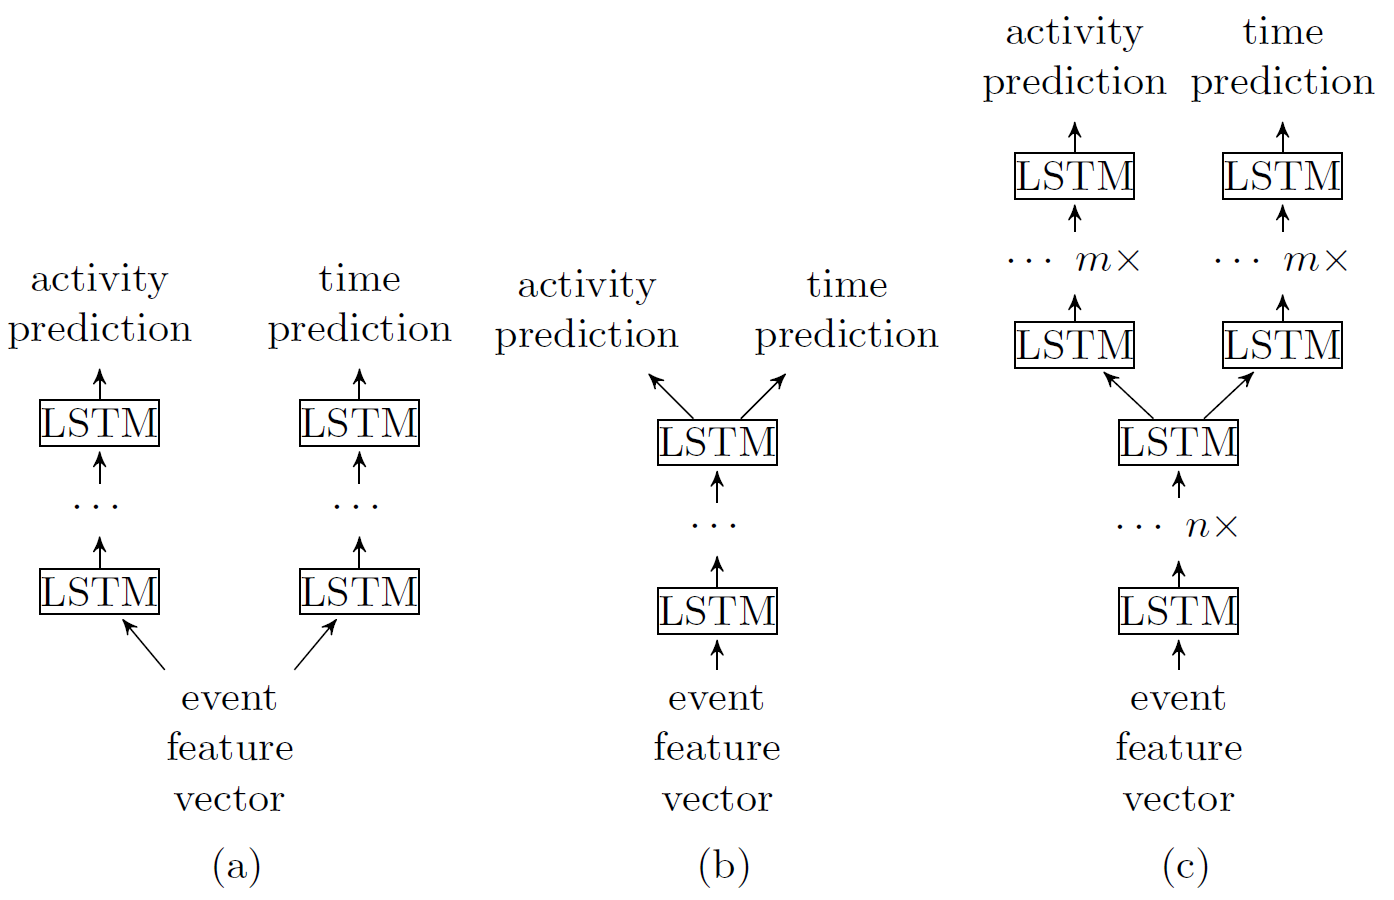
\includegraphics[width=\textwidth]{1.png}
		\caption{Possible neural network architectures \cite{niek96732}. Single task layers (a), shared multitask layers (b), or n+m shared layers (c).}
		\label{figure:architectureslstm}	
	\end{center}
\end{figure}


The evaluation was done on many data sets, such as Helpdesk, BPI12, BPI12 with no duplicates, Environment permit. On most of them suffix (sequence of next events) prediction beats state of the art performance. It worked especially well with logs that had a lot of short traces (Helpdesk log contains average 7 event traces).

The problem investigated in this paper falls best into the problems discussed in this section i.e., into the set of very recent efforts aiming at predicting the sequence of future activities given the activities observed so far.

%In~\cite{Maggi:CAiSE2014} a framework is introduced, which is able to predict the fulfillment (or the violation) of a boolean predicate in a running case, by looking at: (i) the sequence of activities already performed in the case; and (ii) the data payload of the last activity of the running case. The framework, which provides accurate results at the expense of a high runtime overhead, has been enhanced in~\cite{Di-Francescomarino:2016aa} by introducing a clustering preprocessing step in which cases sharing a similar activity history are clustered together. A classifier for each cluster is trained with the data payload of the traces in the cluster. In~\cite{Leontjeva2015}, the authors compare different feature encoding approaches where traces are treated as complex symbolic sequences, that is, sequences of activities each carrying a data payload consisting of attribute-value pairs. In~\cite{DBLP:conf/bpm/TeinemaaDMF16}, the unstructured information contained in text messages exchanged during process executions has been leveraged for improving the prediction accuracy.


%~\cite{Polatoetal:2016,niek96732,evermann}.
%In~\cite{Polatoetal:2016}, Polato et al.~propose several techniques for predicting the remaining time and the sequence of future activities in an ongoing case using simple regression, regression with contextual information, and data-aware transition systems.
%
%Recently, many machine learning toolkits started leveraging the power
%of Graphical Processing Units (GPUs).  This allowed researchers and
%engineer to train their NNs in a significantly reduced amount of time:
%many complex network architectures have been trained to perform
%several task, many of them achieving remarkable performances.  Such
%innovation fostered a new interest in NNs that spread across both
%Industry and Industry.  Business Process Management is not an
%exception. \cite{quteprints96732,niek96732,evermann} Recent papers
%suggest state of the art performance on the prediction tasks for
%business process log outcomes.
%
%Due to the nature of the problem, that is the sequence to sequence prediction, the recurrent neural networks are most leveraged. The main motivation for this type of neural networks is currently the problems in Natural Language Processing, such as speech recognition\cite{graves2013icassp}, or translation\cite{Sutskever2014SSL29690332969173}.
%


%\todoincg{Fix bibentry for Niek. I would cite the technical report from which we took the data adding as a note that a version is to appear in CAISE 2017.}

%They achieve state of the art performance on most logs evaluated.
%In order to predict the next events and their timestamps, they rely on a boolean encoding of the event sequences and on few time-related features. The encoding is then used for feeding the RNN.

%In order to predict next event and time, they use one-hot encoding for event sequence, and few time features (such as difference between time-stamps, time from midnight, time from beginning of the week). Using these features they construct a vector to be fed into recurrent neural network.

%They are looking for functions $f_a^1$ and $f_t^1$ that are basically the probability distributions over all possible trace continuations.

%Also, as they now have basically two sequences to train with, that are the sequence of events, and the sequence of time values, the paper suggests the different possible RNN architectures.
%\begin{figure}[!ht]
%	\begin{center}
%		\includegraphics[width=\textwidth]{paper1233.png}
%		\caption{Possible neural network architectures \cite{niek96732}. Single task layers (a), shared multitask layers (b), or n+m shared layers (c).}
%	\end{center}
%\end{figure}

%The evaluation was done on many data sets, such as Helpdesk, BPI12, BPI12 with no duplicates, Environment permit. On most of them suffix (sequence of next events) prediction beats state of the art performance. It worked especially well with logs that had a lot of short traces (Helpdesk log contains average 7 event traces).
%%% Local Variables:
%%% mode: latex
%%% TeX-master: "BPM17"
%%% End:
